% $Id: INF_Poster_example.tex 7714 2011-08-31 17:34:46Z tkren $
%
% TU Wien - Faculty of Informatics
% poster template
%
% This template is using the beamer document class and beamerposter package, see
% <http://www.ctan.org/tex-archive/macros/latex/contrib/beamer/>
% <http://www.ctan.org/tex-archive/macros/latex/contrib/beamerposter/>
% <http://www-i6.informatik.rwth-aachen.de/~dreuw/latexbeamerposter.php>
%
% For questions and comments send an email to
% Thomas Krennwallner <tkren@kr.tuwien.ac.at>
%

\documentclass[final,hyperref={pdfpagelabels=true}]{beamer}

\usepackage{TUINFPST}   			% Poster template
\usepackage{algorithm}  			% For algorithms
\usepackage[noend]{algpseudocode} 	% Allows pseudo-code like syntax in algorithms
\usepackage{caption}				% Better caption handling

%\title[Computational Intelligence]{Interactive Computer Generated Architecture}
% if you have a long title looking squeezed on the poster, just force
% some distance:
\title[\protect\parbox{.65\textwidth}{Software Engineering \& Internet Computing}]{%
  Context Enrichment of \\[0.2\baselineskip]%
  Crowdsourcing Tasks for \\[0.2\baselineskip]%
  Ontology Validation
}
\author[stefan.gamerith@gmx.com]{Stefan Gamerith}
\institute[]{%
  Technische Universit{\"a}t Wien\\[0.25\baselineskip]
  Institut f{\"u}r Softwaretechnik und Interaktive Syteme\\[0.25\baselineskip]
  Arbeitsbereich: Information \& Software Engineering Group\\[0.25\baselineskip]
  Betreuer: Ao.Univ.-Prof. Dr. techn. Stefan Biffl\\[0.25\baselineskip]
  Mitwirkung: MSc., PhD Marta Reka Sabou
}
\titlegraphic{
\includegraphics[height=52mm]{logo_ifs_cmyk}}
\date[\today]{\today}
\subject{epilog}
\keywords{my kwd1, my kwd2}

%%%%%%%%%%%%%%%%%%%%%%%%%%%%%%%%%%%%%%%%%%%%%%%%%%%%%%%%%%%%%%%%%%%%%%%%%%%%%%%%%%%%%%

% Display a grid to help align images 
%\beamertemplategridbackground[12.7mm]

% play around with the background colors
% \setbeamercolor{background canvas}{bg=yellow}

% use a background picture
% \usebackgroundtemplate{%
%   
\includegraphics[width=\paperwidth]{logo_KBS_2_CMYK}
% }

%CAPTION SETUP
\captionsetup[algorithm]{font=footnotesize}

%ADJUST MARGIN%
\setbeamersize{text margin left=12.7mm,text margin right=12.7mm} 
\setlength{\textwidth}{811.8mm}

% BLOCK COLORS
\setbeamercolor{block body}{fg=black,bg=InfosysVeryLightGrey}
\setbeamercolor{block title}{fg=white,bg=TuWienBlueLight}

% BEGIN BLOCK TEMPLATE %
\setbeamertemplate{block begin}{
  \begin{beamercolorbox}{block title}%
        \begin{minipage}[c][2cm]{\textwidth}
          \centering\textbf{\insertblocktitle}
        \end{minipage}
  \end{beamercolorbox}
  {\ifbeamercolorempty[bg]{block body}{}{\nointerlineskip}}%
	  \begin{beamercolorbox}[leftskip=1em,sep=1ex,vmode]{block body}%
}

% END BLOCK TEMPLATE %
\setbeamertemplate{block end}{
  \end{beamercolorbox}
  \vspace{2cm}
}

% for crop marks, uncomment the following line
%\usepackage[cross,width=88truecm,height=123truecm,center]{crop}

%%%%%%%%%%%%%%%%%%%%%%%%%%%%%%%%%%%%%%%%%%%%%%%%%%%%%%%%%%%%%%%%%%%%%%%%%%%%%%%%%%%%%%
\begin{document}

\begin{frame}
  \begin{columns}[t, onlytextwidth]

    \begin{column}{\textwidth}
		
		%TOP%
		\begin{columns}[t, onlytextwidth]
			
			\begin{column}{.49\linewidth}
				\begin{block}{Context \& Motivation}
					\begin{minipage}{.45\linewidth}
						\begin{figure}
							\centering
							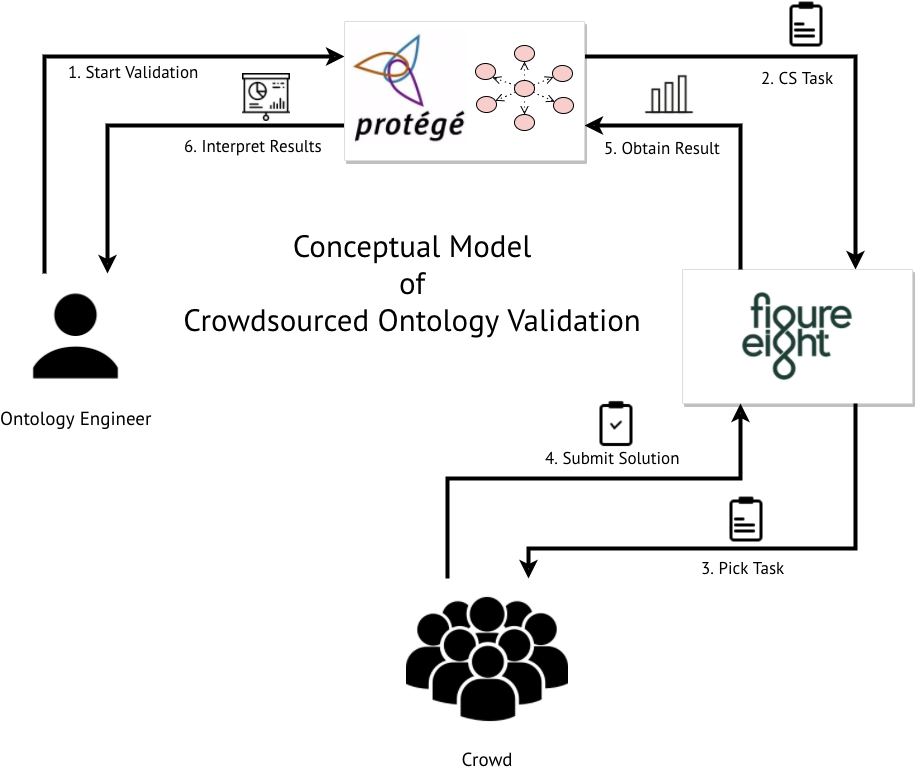
\includegraphics[width=\textwidth]{figures/model_ontology_validation}
						\end{figure}
					\end{minipage}
					\hfill
					\begin{minipage}{.45\linewidth}
						\small
						{\color{BeamerBlue}{Crowdsourced Ontology Validation}}
						uses Human Computation to validate ontologies in a cost effective way. 
						\vspace{1.5cm}
						
						The {\color{BeamerBlue}{uComp Protege Plugin}} allows the
						creation and execution of Crowdsourcing~(CS) tasks for ontology validation from within the Protege ontology editor.
						\vspace{1.5cm}
						
						{\color{BeamerBlue}{Problem:}} Crowd workers often do not had enough Context to complete such CS tasks.
						\vspace{1.5cm}
						
						{\color{BeamerBlue}{Solution:}} Extend plugin to enrich CS tasks with Context.
						\vspace{1.5cm}
					\end{minipage}
					\hfill
				\end{block}
			\end{column}
			
			\begin{column}{.49\linewidth}
				\begin{block}{Research Questions}
					    \begin{itemize}
							\setlength\itemsep{1.5cm}
					    	\item \textsc{\color{BeamerBlue}{Context Enrichment of Crowdsourcing Tasks}}
							
							Does the crowd perform better on context enriched Crowdsourcing tasks?
					    	\item \textsc{\color{BeamerBlue}{Context Enrichment Methods}}
							
							What methods can be applied that generate Context?
					    	\item \textsc{\color{BeamerBlue}{Generalising the Applicability of the proposed Methods}}
							
							To what extent is it possible to transfer the investigated methods to different datasets?
					    	\item \textsc{\color{BeamerBlue}{Comparative Evaluation of the proposed Methods}}
							
							Which of the proposed methods works best? What are potential shortcomings and why?
					    \end{itemize}
				\end{block}
			\end{column}
			
		\end{columns}
		
		%MIDDLE%
		%
		% APPROACH FEATURES:
		%	First Headline
		%   Second Headline
		%   Precondition
		%   Strengths
		%   Weaknesses
		\begin{column}{\textwidth}
			\begin{block}{Context Enrichment Methods}
			    \begin{minipage}[t]{.3\linewidth}
					\begin{center}
						\textsc{\color{BeamerBlue}{Ontology based Approach}}
					\end{center}
					\vspace{1cm}
					\begin{algorithm}[H]
						\footnotesize
						\caption{\parbox[c][2cm][c]{\textwidth}{Context Generation based on Neighbouring Nodes}}
						\vspace{5mm}
						\begin{algorithmic}
							\Procedure{Generate Description}{}\newline
								\textbf{Input:} A concept $C$\newline
								\textbf{Output:} A textual description $T$ of $C's$ neighbouring nodes based on subsumption\newline
								\State{$T=\{\}$}
								\For {$ (c,d) \in C \sqsubseteq D $}
									\State $T=T$ $\cup$ "Every " $\cup$ $name(c)$ $\cup$ " is a " $\cup$ $name(d)$
								\EndFor
								\For {$ (e,c) \in E \sqsubseteq C $}
									\State $T=T$ $\cup$ "Every " $\cup$ $name(e)$ $\cup$ " is a " $\cup$ $name(c)$
								\EndFor
							\EndProcedure
						\end{algorithmic}
						\vspace{5mm}
					\end{algorithm}
					\vspace{1cm}
					\begin{itemize}
						\small
						\setlength\itemsep{0.5cm}
						\item Context Generation based on {\color{BeamerBlue}{Subsumption Relations}}
						\item The algorithm outputs {\color{BeamerBlue}{ACE~(Attempto Controlled English)}} texts
						\item {\color{BeamerBlue}{Fully automated}} without external dependencies
						\item Achieves its {\color{BeamerBlue}{strengths}} in compact, tightly connected ontologies
						\item Just a subset of ACE rules were implemented
					\end{itemize}
					\vspace{1.5cm}
				\end{minipage}
				\hfill\vline\hfill
			    \begin{minipage}[t]{.3\linewidth}
					\begin{center}
						\textsc{\color{BeamerBlue}{Metadata based Approach}}						
					\end{center}
					\vspace{1cm}
					\begin{algorithm}[H]
						\footnotesize
						\caption{\parbox[c][2cm][c]{\textwidth}{Context Generation based on Embedded Metadata}}
						\vspace{5mm}
						\begin{algorithmic}
							\Procedure{Generate Description}{}\newline
								\textbf{Input:} A concept $C$ with embedded metadata $\{m_1, m_2, \ldots, m_i \}$\newline
								\textbf{Output:} A description $T$ of $C's$ metadata elements\newline
								\State{$T=\{\}$}
								\For {$ m_k \in \Phi(C) $}
									\State $T=T$ $\cup$ $m_k$
								\EndFor
							\EndProcedure
						\end{algorithmic}
						\vspace{5mm}
					\end{algorithm}
					\vspace{1cm}
					\begin{itemize}
						\small
						\setlength\itemsep{1.15cm}
						\item Context Generation based on {\color{BeamerBlue}{Annotation Properties}}
						\item Terms of the {\color{BeamerBlue}{Dublin Core Metadata Set}} were used to encode the metadata
						\item The metadata needs to be {\color{BeamerBlue}{added manually}} by (domain)~experts beforehand
						\item Gives the {\color{BeamerBlue}{most control}} over Context Generation
						\item Requires the most human involvement
					\end{itemize}
				\end{minipage}
				\hfill\vline\hfill
			    \begin{minipage}[t]{.3\linewidth}
					\begin{center}						
						\textsc{\color{BeamerBlue}{Dictionary based Approach}}
					\end{center}
					\vspace{1cm}
					\begin{figure}[H]
						 \centering
						 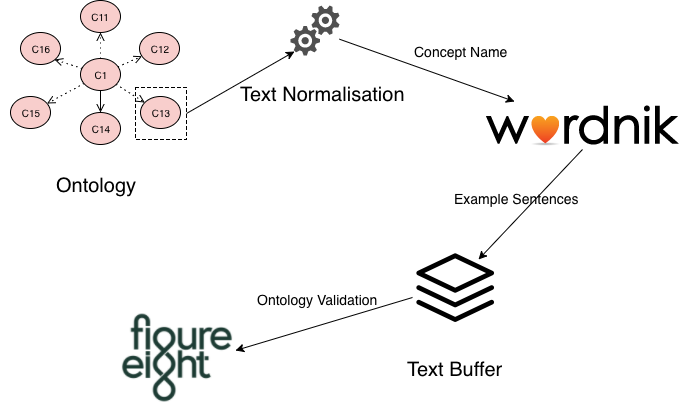
\includegraphics[width=\textwidth]{figures/External_Source_Workflow}
						 \caption{Conceptual Model of WordNik consultation to generate Context}
					\end{figure}
					\vspace{-1cm}
					\hrulefill
					\vspace{1.5cm}
					\begin{itemize}
						\small
						\setlength\itemsep{0.5cm}
						\item Context Generation based on {\color{BeamerBlue}{Dictionary Lookup}}
						\item Fetches Context from the online dictionary {\color{BeamerBlue}{WorkNik}}
						\item Has its {\color{BeamerBlue}{strengths}} when ontologies contain common, well known concepts
						\item Fails when concept names contain phrases or special characters
					\end{itemize}
					\vspace{1.5cm}
				\end{minipage}
				\hfill
			\end{block}
		\end{column}
		
		
		%BOTTOM%
		\begin{columns}[t, onlytextwidth]
			\begin{column}{.49\linewidth}
				\begin{block}{Experimental Evaluation}
					    Lorem ipsum dolor sit amet, consectetur adipisicing elit, sed do eiusmod tempor incididunt ut labore et dolore magna aliqua. Ut enim ad minim veniam, quis nostrud exercitation ullamco laboris nisi ut aliquip ex ea commodo consequat. Duis aute irure dolor in reprehenderit in voluptate velit esse cillum dolore eu fugiat nulla pariatur. Excepteur sint occaecat cupidatat non proident, sunt in culpa qui officia deserunt mollit anim id est laborum.
				\end{block}
			\end{column}
			\begin{column}{.49\linewidth}
				\begin{block}{Improvements through Context Enrichment}
					    Lorem ipsum dolor sit amet, consectetur adipisicing elit, sed do eiusmod tempor incididunt ut labore et dolore magna aliqua. Ut enim ad minim veniam, quis nostrud exercitation ullamco laboris nisi ut aliquip ex ea commodo consequat. Duis aute irure dolor in reprehenderit in voluptate velit esse cillum dolore eu fugiat nulla pariatur. Excepteur sint occaecat cupidatat non proident, sunt in culpa qui officia deserunt mollit anim id est laborum.
				\end{block}
			\end{column}
		\end{columns}
		
    \end{column}

  \end{columns}
\end{frame}


\end{document}
